% Scalar instruction entry source: tools/generate_scalar_instruction_catalog.py.
\subsection{\texttt{LUI}}
\label{sec:scalar-lui}
\index{LUI@\texttt{LUI}}
\begin{sloppypar}\noindent\textbf{Purpose.} Load upper immediate (constant materialization).\end{sloppypar}\smallskip
\noindent\textbf{Syntax.}\par
\begin{lstlisting}[style=ptoscalarcode]
lui simm, ->RegDst
\end{lstlisting}
\noindent\textbf{Encoding.}\par
\noindent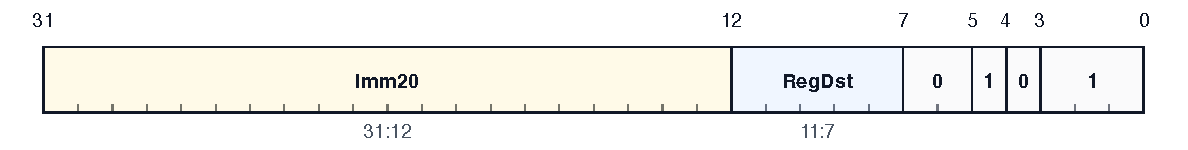
\includegraphics[width=\textwidth]{figs/encoding/scalar_instruction_entries/enc_lui.pdf}\par\smallskip
\begin{description}[leftmargin=0.18\linewidth,style=nextline]
\item[Format] \texttt{L32} \texttt{32-bit} scalar word.
\item[Pattern] \texttt{.........................0010111}.
\end{description}
\noindent\textbf{Classification.}\par
\begin{description}[leftmargin=0.18\linewidth,style=nextline]
\item[Category] Integer ALU and Bit-Manipulation.
\item[Family] Immediate.
\item[Execution class] \texttt{ALU}; uop\_kind=ALU.
\end{description}
\noindent\textbf{Operand fields.}\par
\begin{description}[leftmargin=0.18\linewidth,style=nextline]
\item[\texttt{RegDst}] Bits \texttt{11:7 (5b)}. 5-bit scalar destination register that receives the loaded value after any sign or zero extension; X0 discards the load result.
\item[\texttt{imm20}] Bits \texttt{31:12 (20b)}. 20-bit unsigned immediate operand consumed directly by the operation.
\end{description}
\noindent\textbf{Operation.}\par
\begin{lstlisting}[style=ptoscalarcode]
imm = (SignExtend(imm20) << 12)
Write(RegDst, imm)
\end{lstlisting}
\Needspace{0.08\textheight}
